\documentclass[tikz, border=10pt]{standalone}
\usetikzlibrary{automata, positioning, arrows}

\begin{document}

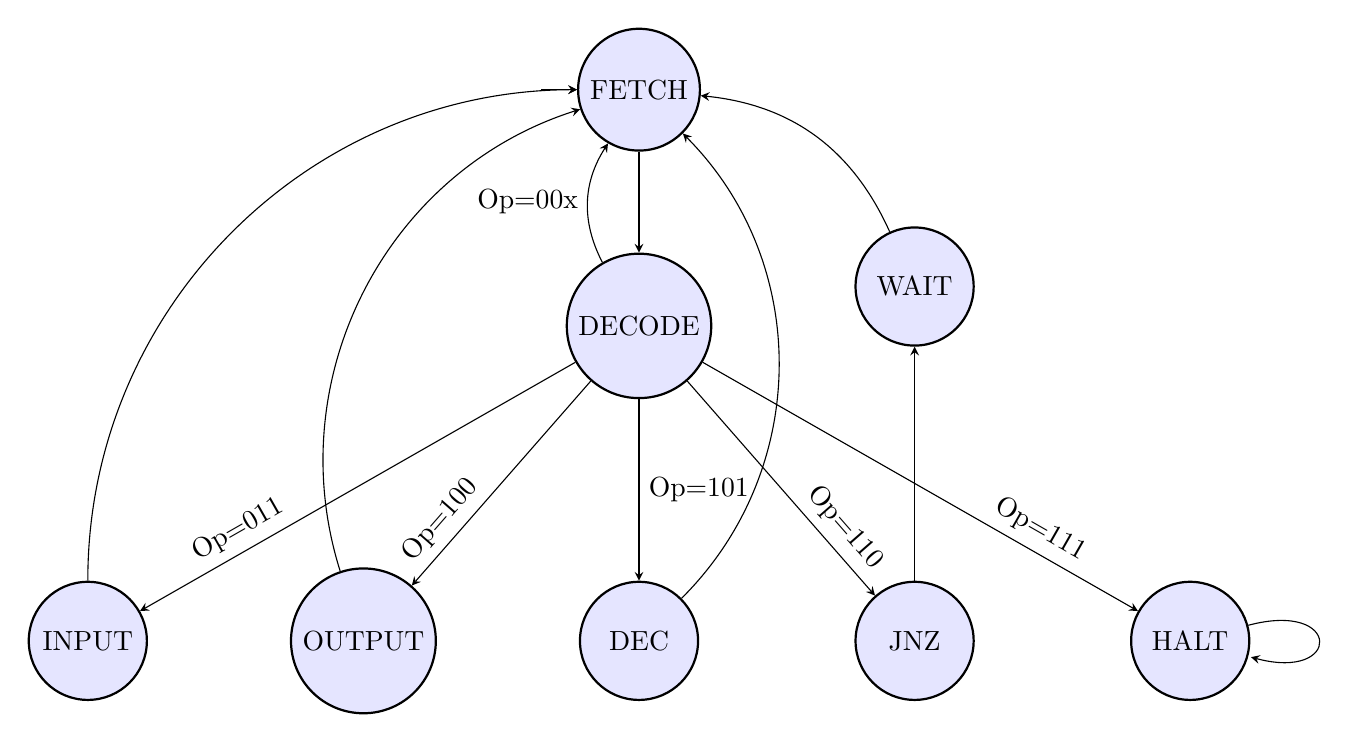
\begin{tikzpicture}[
    ->, >=stealth, auto, node distance=2.5cm,
    every state/.style={thick, fill=blue!10, minimum size=1.5cm},
    initial text=$ $
]

    % Top Level
    \node[state, initial] (FETCH) {FETCH};
    
    % Second Level
    \node[state, below of=FETCH, node distance=3cm] (DECODE) {DECODE};
    
    % Bottom Level (Operations)
    \node[state, below of=DECODE, node distance=4cm] (DEC) {DEC};
    \node[state, left of=DEC, node distance=3.5cm] (OUTPUT) {OUTPUT};
    \node[state, left of=OUTPUT, node distance=3.5cm] (INPUT) {INPUT};
    \node[state, right of=DEC, node distance=3.5cm] (JNZ) {JNZ};
    \node[state, above of=JNZ, node distance=4.5cm] (WAIT) {WAIT};
    \node[state, right of=JNZ, node distance=3.5cm] (HALT) {HALT};

    % Edges
    % Fetch -> Decode
    \path (FETCH) edge node {} (DECODE);
    
    % Decode -> Operations
    \path (DECODE) edge node [above, sloped,near end] {Op=011} (INPUT)
          (DECODE) edge node [above, sloped, near end] {Op=100} (OUTPUT)
          (DECODE) edge node {Op=101} (DEC)
          (DECODE) edge node [above, sloped, near end] {Op=110} (JNZ)
          (DECODE) edge node [above, sloped,near end] {Op=111} (HALT);
          
    % NOP: Decode -> Fetch
    \path (DECODE) edge [bend left=30, align=center] node [left] {Op=00x} (FETCH);

    % Operations -> Fetch (Return)
    \path (INPUT)  edge [bend left=45] node {} (FETCH)
          (OUTPUT) edge [bend left=45] node {} (FETCH)
          (DEC)    edge [bend right=45]  node {} (FETCH) % Slightly offset to avoid overlapping straight line
          (JNZ)    edge node {} (WAIT)
          (WAIT)   edge [bend right] node {} (FETCH);
          
    % Halt Loop
    \path (HALT)   edge [loop right] node {} (HALT);

\end{tikzpicture}

\end{document}
